
This setup is based on a poster by Quinquis et al, presented at EGU 2010. 

The domain is 2680x670km, i.e. aspect ratio is exactly 4.
Boundary conditions are free slip left, bottom and top. 
A horizontal velocity profile is prescribed on the right boundary, but 
only the horizontal component is prescribed. 


\begin{center}
\includegraphics[width=12cm]{python_codes/fieldstone_67/images/setup}
\end{center}

There are 7 materials in the domain:
\begin{center}
\includegraphics[width=7cm]{python_codes/fieldstone_67/images/mats}
\includegraphics[width=7cm]{python_codes/fieldstone_67/images/maats}
\end{center}

Depths of interfaces on the left are 7,39,82km and 8,40,110km on the right.
The opening angle of the circular part is $45\degree$ and the 
already subducted slab (i.e. LH=MI=NJ=OK) is 130km long:

\begin{center}
\includegraphics[width=12cm]{python_codes/fieldstone_67/images/mats3}
\end{center}

The coordinates of points H to O are then as follows:

\begin{lstlisting}
xH=Lx/2-np.sqrt(2.)/2.*200e3 ; yH=Ly-200e3+np.sqrt(2.)/2.*200e3
xI=Lx/2-np.sqrt(2.)/2.*192e3 ; yI=Ly-200e3+np.sqrt(2.)/2.*192e3
xJ=Lx/2-np.sqrt(2.)/2.*160e3 ; yJ=Ly-200e3+np.sqrt(2.)/2.*160e3
xK=Lx/2-np.sqrt(2.)/2.*90e3  ; yK=Ly-200e3+np.sqrt(2.)/2.*90e3
xL=xH-130e3*np.sqrt(2.)/2. ; yL=yH-130e3*np.sqrt(2.)/2.
xM=xI-130e3*np.sqrt(2.)/2. ; yM=yI-130e3*np.sqrt(2.)/2.
xN=xJ-130e3*np.sqrt(2.)/2. ; yN=yJ-130e3*np.sqrt(2.)/2.
xO=xK-130e3*np.sqrt(2.)/2. ; yO=yK-130e3*np.sqrt(2.)/2.
\end{lstlisting}

The velocity profile on the right boundary is described in Section~\ref{kin_bc}, and we 
impose $y_1=L_y-160$km and $y_2=L_y-128$km, and a $u_{in}=5$cm/year.

The mesh is first created so that all elements have the same dimensions $h_x=L_x/nelx$ and $h_y=L_y/nely$.
It is then stretched using the two functions {\sl stretch\_towards\_center} and 
{\sl stretch\_towards\_top}.


\begin{center}
\includegraphics[width=7cm]{python_codes/fieldstone_67/images/vel}
\includegraphics[width=7cm]{python_codes/fieldstone_67/images/vel2}\\
\includegraphics[width=7cm]{python_codes/fieldstone_67/images/eta}
\includegraphics[width=7cm]{python_codes/fieldstone_67/images/rho}\\
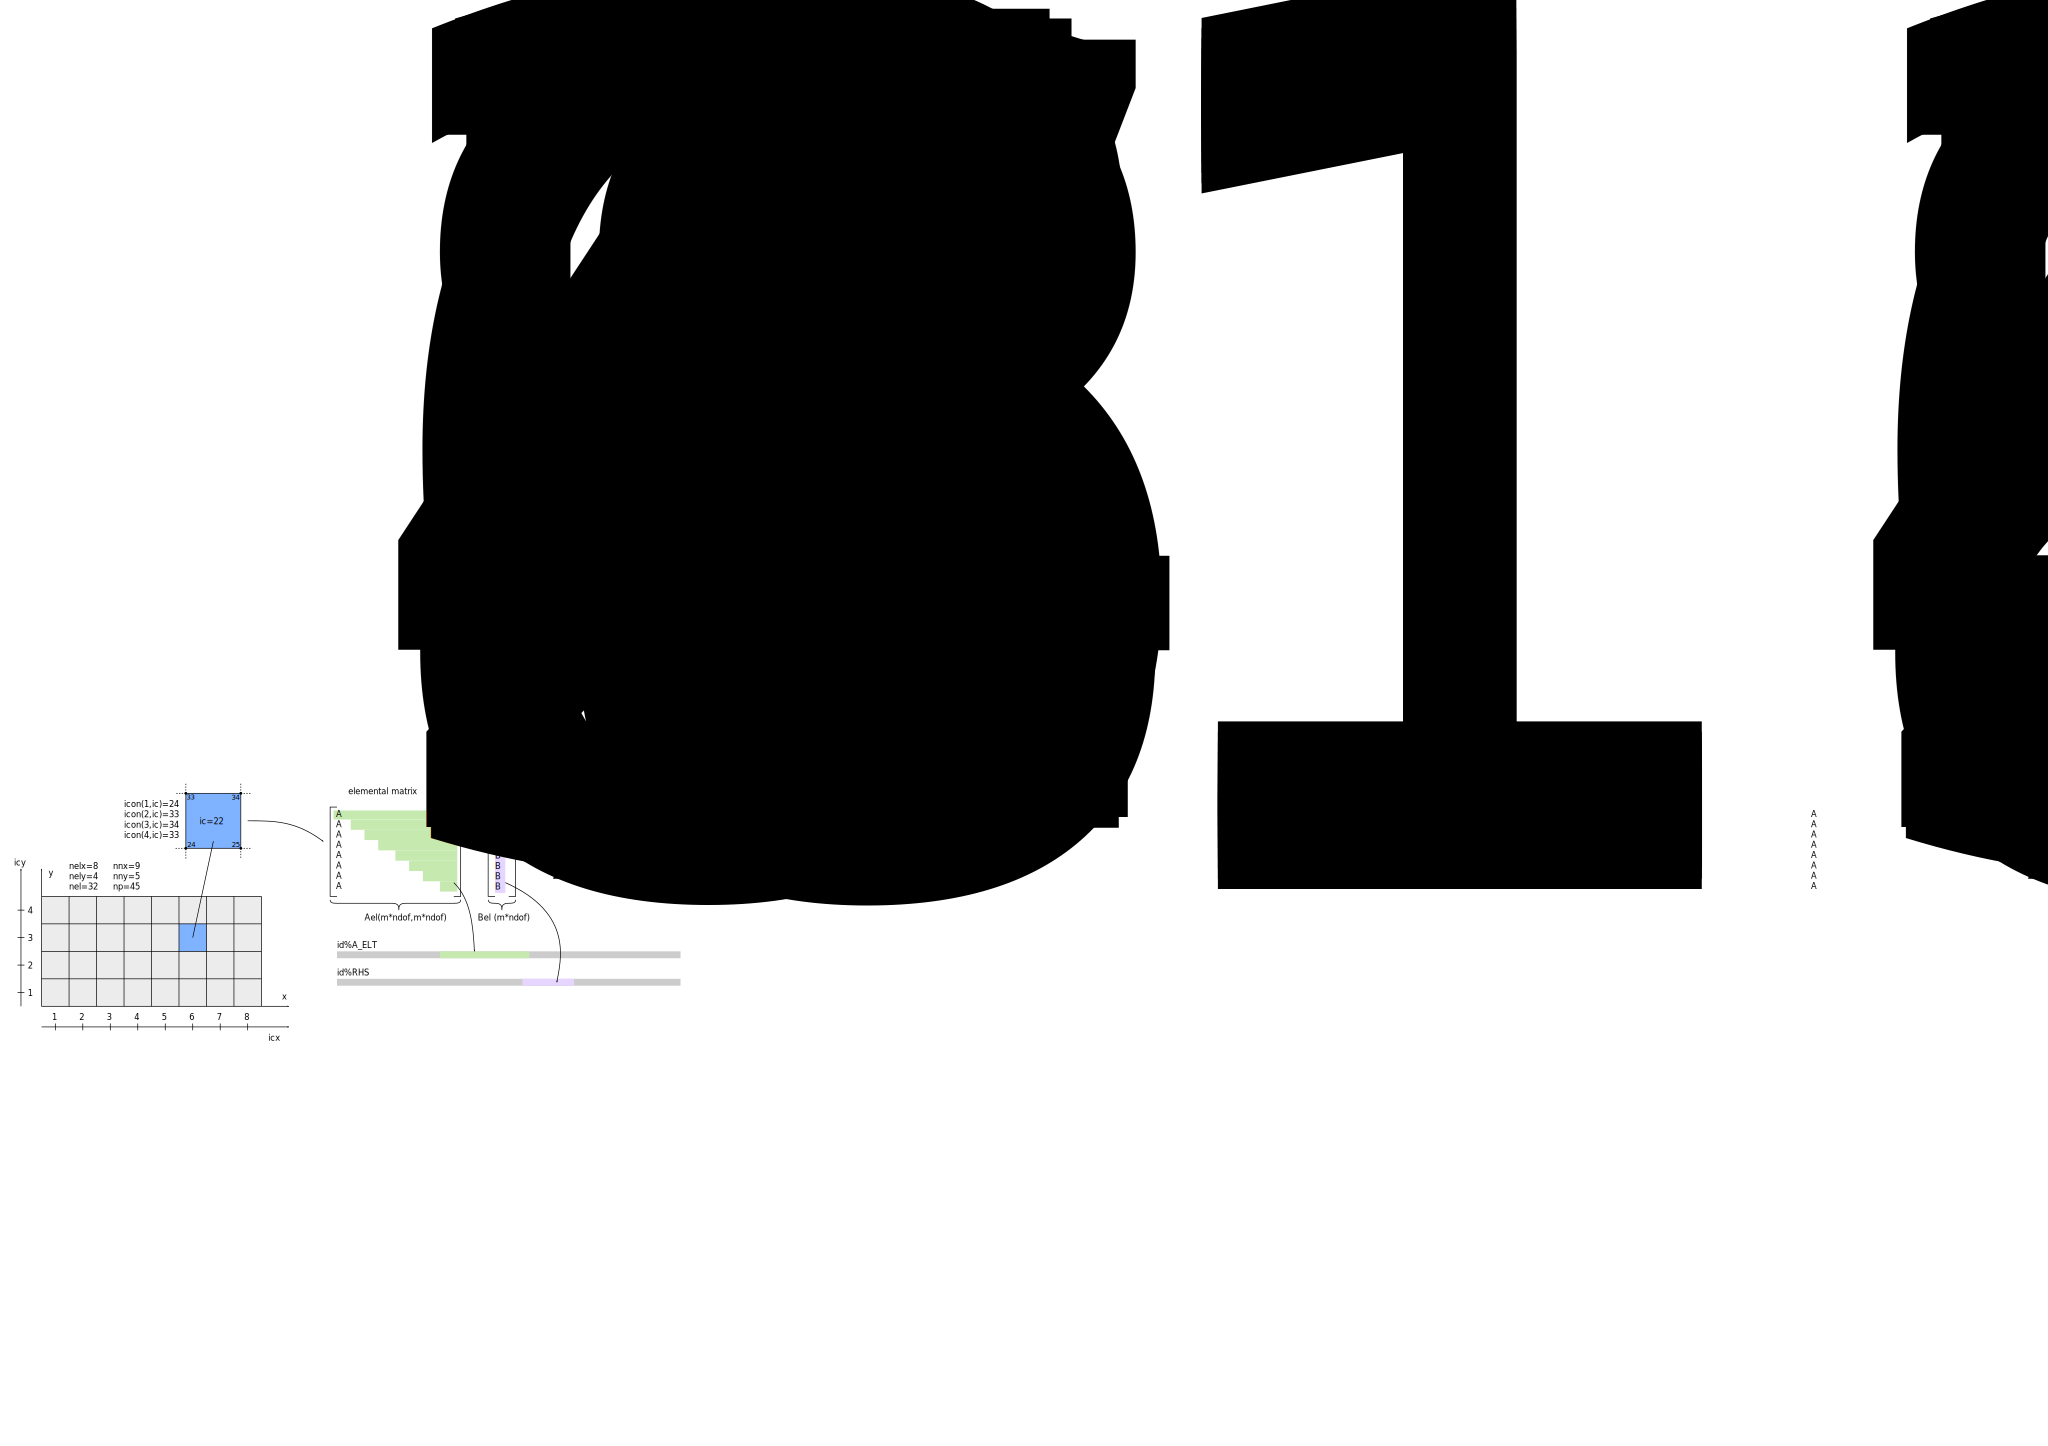
\includegraphics[width=7cm]{python_codes/fieldstone_67/images/grid}
\includegraphics[width=7cm]{python_codes/fieldstone_67/images/sr}\\
{\captionfont 256x64 elements with mesh stretching. Viscosity averaging is harmonic.
Density averaging is arithmetic.}
\end{center}

COMPUTE ANALYTICAL MASS ?!
